\documentclass[amscd, amssymb, verbatim]{amsart}[12pt]

\usepackage{fullpage}
\usepackage{amssymb}
\usepackage{latexsym}
\usepackage{pb-diagram}
\usepackage[mathscr]{euscript}
\usepackage{graphicx}
\usepackage{subfigure}
\usepackage{placeins}
\usepackage{wrapfig}
\usepackage{url}
\usepackage{appendix}
\usepackage{multind}
\makeindex{1}

\theoremstyle{remark}
\newtheorem{exercise}{Exercise}[subsection]
\newcommand{\lc}{\lowercase}
\errorcontextlines=0
\newcommand{\comment}[1]{}

\setlength{\parindent}{0pt}

\begin{document}

\title{J\lc{ava}P\lc{lex} T\lc{utorial}}
\author{H\lc{enry} A\lc{dams and} A\lc{ndrew} T\lc{ausz} \\ \lc{henrya@math.stanford.edu and atausz@stanford.edu} \\ M\lc{ay 22, 2011}}


\maketitle

% for javaplex.jar 5/20/11 7:14 PM

% remove \index{}

\tableofcontents




\section{Introduction}

%\subsection{JPlex}\label{jplexIntro}
%JPlex is a Java software package for computing the persistent homology of filtered simplicial complexes, often generated from point cloud data. The authors are Harlan Sexton and Mikael Vejdemo Johansson. This is a tutorial for using JPlex with Matlab. There is a similar document for using JPlex with BeanShell. Please email me (\texttt{henrya@math.stanford.edu}) with questions about this tutorial. Some of the exercises are borrowed from Vin de Silva's {\em Plexercises} (\url{http://comptop.stanford.edu/u/programs/Plexercises2.pdf}). Other sources of information about JPlex are the javadoc tree for the JPlex library (\url{http://comptop.stanford.edu/programs/jplex/files/javadoc/index.html}) and the TMSCSCS website (\url{http://comptop.stanford.edu/programs/}). \\

\subsection{JavaPlex}\label{javaplexIntro}

JavaPlex is a Java software package for computing the persistent homology of filtered chain complexes, with special emphasis on applications arising in topological data analysis. The main author is Andrew Tausz. JavaPlex is a re-write of the JPlex package, which was written by Harlan Sexton and Mikael Vejdemo Johansson. The main motivation for the development of JavaPlex was the need for a flexible platform that supported new directions of research in topological data analysis and computational persistent homology. The website for JavaPlex is \url{http://code.google.com/p/javaplex/} and the javadoc tree for the library can be found at \url{http://javaplex.googlecode.com/svn/trunk/doc/index.html}. \\

If you are interested in JavaPlex, then you may also be interested in the software package Dionysus by Dmitriy Morozov, available at \url{http://www.mrzv.org/software/dionysus}. \\

\subsection{License}\label{license}

JavaPlex is an open source software package under the Open BSD License. The source code can be found at \url{http://code.google.com/p/javaplex/}. If you are interested in contributing to the project, we invite you to contact either of the authors. \\

\subsection{Installation for Matlab}\label{install}
Open Matlab and check which version of Java is being used. In this tutorial, the symbol \texttt{>>} precedes commands to enter into your Matlab window.
\begin{quote} \texttt{>> version -java \\
ans = Java 1.5.0\_13 with Apple Inc.   Java Hotspot(TM) Client VM mixed mode, sharing
} \end{quote}
JavaPlex requires version number \texttt{1.5} or higher. \\ % CONFIRM

**** Explain how to download and extract % TODO

Extract the contents of the zip file containing the examples. It should be called something like \texttt{javaplex-examples-4.00.tar.gz}. 

%Copy \texttt{plex.jar} into a directory of your choice. If you choose the current Matlab directory, then you do not need to edit m-file \texttt{load\_javaplex.m} and can skip the rest of this paragraph. Suppose instead you have chosen the directory \texttt{/Users/myName/}. Open the m-file \texttt{load\_javaplex.m}, which contains the following lines.
%\begin{quote} \texttt{javaaddpath('plex.jar') \\
%import edu.stanford.math.plex.*;} \end{quote}
%Replace \texttt{'plex.jar'} above with \texttt{'/Users/myName/plex.jar'} (substitute the path of your chosen directory). Save \texttt{load\_javaplex.m}. \\

Run the \texttt{load\_javaplex.m} file. 
\begin{quote} \texttt{>> load\_javaplex
} \end{quote}
%Installation is complete. Confirm that JavaPlex is working properly with the following command.
%\begin{quote} \texttt{ >> homology.chain\_basis.Simplex.makeSimplex(4)\\
%ans =[4]
%} \end{quote}
Each time upon starting a new Matlab session, you will need to run \texttt{load\_javaplex.m}. \\

\subsection{Accompanying files}\label{accompany}

Matlab scripts containing the commands in this tutorial are available in the folder \texttt{javaplex/src/matlab/for\_distribution/tutorial\_examples}. \\

%TODO




\section{Math review}

Below is a brief math review. For more details, see \cite{a83, eh10, h02, zc05}. 

\subsection{Simplicial complexes}
An abstract simplicial complex is given by the following data.
\begin{itemize}
\item A set $Z$ of vertices or 0-simplices.
\item For each $k\geq 1$, a set of $k$-simplices $\sigma = [z_0z_1...z_k]$, where $z_i\in Z$.
\item Each $k$-simplex has $k+1$ faces obtained by deleting one of the vertices. The following membership property must be satisfied: if $\sigma$ is in the simplicial complex, then all faces of $\sigma$ must be in the simplicial complex.
\end{itemize}
We think of 0-simplices as vertices, 1-simplices as edges, 2-simplices as triangular faces, and 3-simplices as tetrahedrons. \\

\subsection{Homology}
Betti numbers help describe the homology of a simplicial complex $X$. The value $Betti_k$, where $k\in \mathbb{N}$, is equal to the rank of the $k$-th homology group of $X$. Roughly speaking, $Betti_k$ gives the number of $k$-dimensional holes. In particular, $Betti_0$ is the number of connected components. For instance, a $k$-dimensional sphere has all Betti numbers equal to zero except for $Betti_0 = Betti_k = 1$. \\

\subsection{Filtered simplicial complexes}
A filtration on a simplicial complex $X$ is a collection of subcomplexes $\{X(t) \ |\ t\in \mathbb{R}\}$ of $X$ such that $X(t) \subset X(s)$ whenever $t\leq s$. The filtration time of a simplex $\sigma \in X$ is the smallest $t$ such that $\sigma \in X(t)$. In JavaPlex, filtered simplicial complexes (or more generally filtered chain complexes) are called streams. \\

% Introduce filtered chain complexes?

\subsection{Persistent homology}
Betti intervals help describe how the homology of $X(t)$ changes with $t$. A $k$-dimensional Betti interval, with endpoints [$t_{start}$, $t_{end}$), corresponds roughly to a $k$-dimensional hole that appears at filtration time $t_{start}$, remains open for $t_{start} \leq t < t_{end}$, and closes at time $t_{end}$. We are often interested in Betti intervals that persist for a long filtration range. \\

Persistent homology depends heavily on functoriality: for $t\leq s$, the inclusion $i:X(t)\to X(s)$ of simplicial complexes induces a map $i_*:H_k(X(t))\to H_k(X(s))$ between homology groups. \\




\section{Explicit simplex streams}\label{streams}

In JavaPlex, filtered simplicial complexes (or more generally filtered chain complexes) are called streams. The class ExplicitSimplexStream allows one to build a simplicial complex from scratch. In \S \ref{sfpc} we will learn about other automated methods of generating simplicial complexes; namely the Vietoris--Rips, witness, and lazy witness constructions. 

\subsection{Explicit simplex streams and homology}

The Matlab script corresponding to this section is \texttt{explicit\_simplex\_example.m}, which is in the folder \texttt{tutorial\_examples}. You may copy and paste commands from this script into the Matlab window, or you may run the entire script at once with the following command.
\begin{quote} \texttt{>> explicit\_simplex\_example\\
} \end{quote}



{\em Circle example.} Let's build a simplicial complex homeomorphic to a circle. We have three 0-simplices: [0], [1], and [2], and three 1-simplices: [0,1], [0,2], [1,2].

\hspace{2.5in}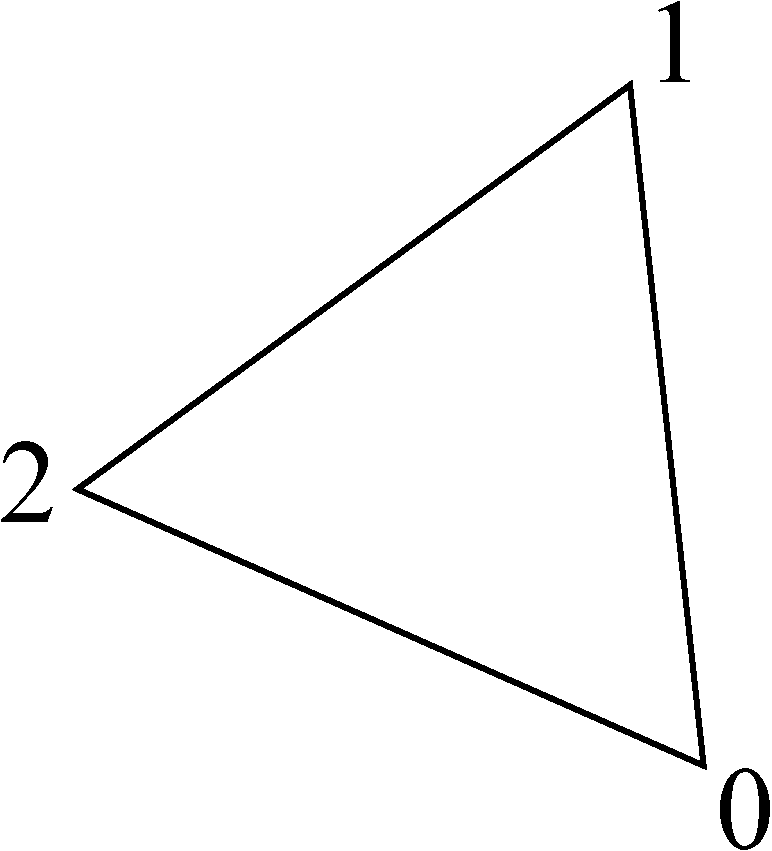
\includegraphics[height=1in]{s1.pdf}

To build a simplicial complex in JavaPlex we simply build a stream in which all filtration times are zero. First we get an empty ExplicitSimplexStream instance. Many command lines in this tutorial will end with a semicolon to supress unwanted output as below.
\begin{quote} \texttt{>> stream = api.Plex4.createExplicitSimplexStream();
} \end{quote}

Next we add simplicies using the methods \texttt{addVertex} and \texttt{addElement}. The first creates a vertex with a specified index, and the second creates a simplex with the given array of vertices. By default, these will all have filtration times of zero.

\begin{quote}\texttt{>> stream.addVertex(0);\\
>> stream.addVertex(1); \\
>> stream.addVertex(2); \\
>> stream.addElement([0, 1]); \\
>> stream.addElement([0, 2]); \\
>> stream.addElement([1, 2]);
} \end{quote}

We print the total number of simplices in the complex.
\begin{quote}\texttt{>> size = stream.getSize() \\
size = 6\\
} \end{quote}

In order to compute the homology of our complex, we first create an object that will perform the computation. The following line obtains the default algorithm for performing simplicial homology. There are other variants on the persistence algorithm, and one can also change the ground field. This default object will perform the homology computation over $\mathbb{Z}/(2)$. The parameter 3 indicates that the maximum dimension to compute homology to is 3. 
\begin{quote}\texttt{>> persistence = api.Plex4.getDefaultSimplicialAlgorithm(3);
} \end{quote}
We compute and print the intervals.
\begin{quote} \texttt{>> triangle\_intervals = persistence.computeIntervals(stream) \\
triangle\_intervals = \\
\\
Dimension: 1 \newline
[0, infinity) \\
\\
Dimension: 0 \newline
[0, infinity)
} \end{quote}
This gives us the expected Betti numbers $Betti_0=1$ and $Betti_1=1$. \\

{\em 9-sphere example.} Let's build a 9-sphere, which is homeomorphic to the boundary of a 10-simplex. First we create a complex containing only a single 10-simplex. This is not a simplicial complex because it does not contain the faces of the 10-simplex. We add all faces using the method \texttt{ensureAllFaces}. Then, we remove the 10-simplex using the method \texttt{removeElementIfPresent}. What remains is the boundary of a 10-simplex, that is, a 9-sphere.

\begin{quote} \texttt{>> stream = api.Plex4.createExplicitSimplexStream();\\
>> dimension = 9;\\
>> stream.addElement(0:(dimension + 1));\\
>> stream.ensureAllFaces();\\
>> stream.removeElementIfPresent(0:(dimension + 1));\\
>> stream.finalizeStream();
}\end{quote}

We print the total number of simplices in the complex.
\begin{quote} \texttt{>> size = stream.getSize()\\
size = 2046
}\end{quote}

We get the default persistence computation
\begin{quote} \texttt{>> persistence = api.Plex4.getDefaultSimplicialAlgorithm(dimension + 1);
}\end{quote}
and compute and print the intervals.
\begin{quote} \texttt{>> n\_sphere\_intervals = persistence.computeIntervals(stream)\\
n\_sphere\_intervals =\\
\\
Dimension: 9\newline
[0, infinity)\\
\\
Dimension: 0\newline
[0, infinity)
} \end{quote}
This gives us the expected Betti numbers $Betti_0=1$ and $Betti_9=1$. \\

\begin{exercise}
Build a simplicial complex homeomorphic to the torus. Compute its Betti numbers. {\em Hint:} You will need at least 7 vertices \cite[page 107]{h02}. We recommend using a $3\times 3$ grid of 9 vertices. \\
\end{exercise}

\begin{exercise}
Build a simplicial complex homeomorphic to the Klein bottle. Check that it has the same Betti numbers as the torus over $\mathbb{Z}_2$ coefficients but different Betti numbers over $\mathbb{Z}_3$ coefficients. \\
\end{exercise}

\begin{exercise}
Build a simplicial complex homeomorphic to the projective plane. Find its Betti numbers over $\mathbb{Z}_2$ and $\mathbb{Z}_3$ coefficients. \\
\end{exercise}


\subsection{Explicit simplex streams and persistent homology}

The Matlab script corresponding to this example is \texttt{house\_example.m}.\\

\begin{wrapfigure}{r}{1in}
	\begin{center}
   	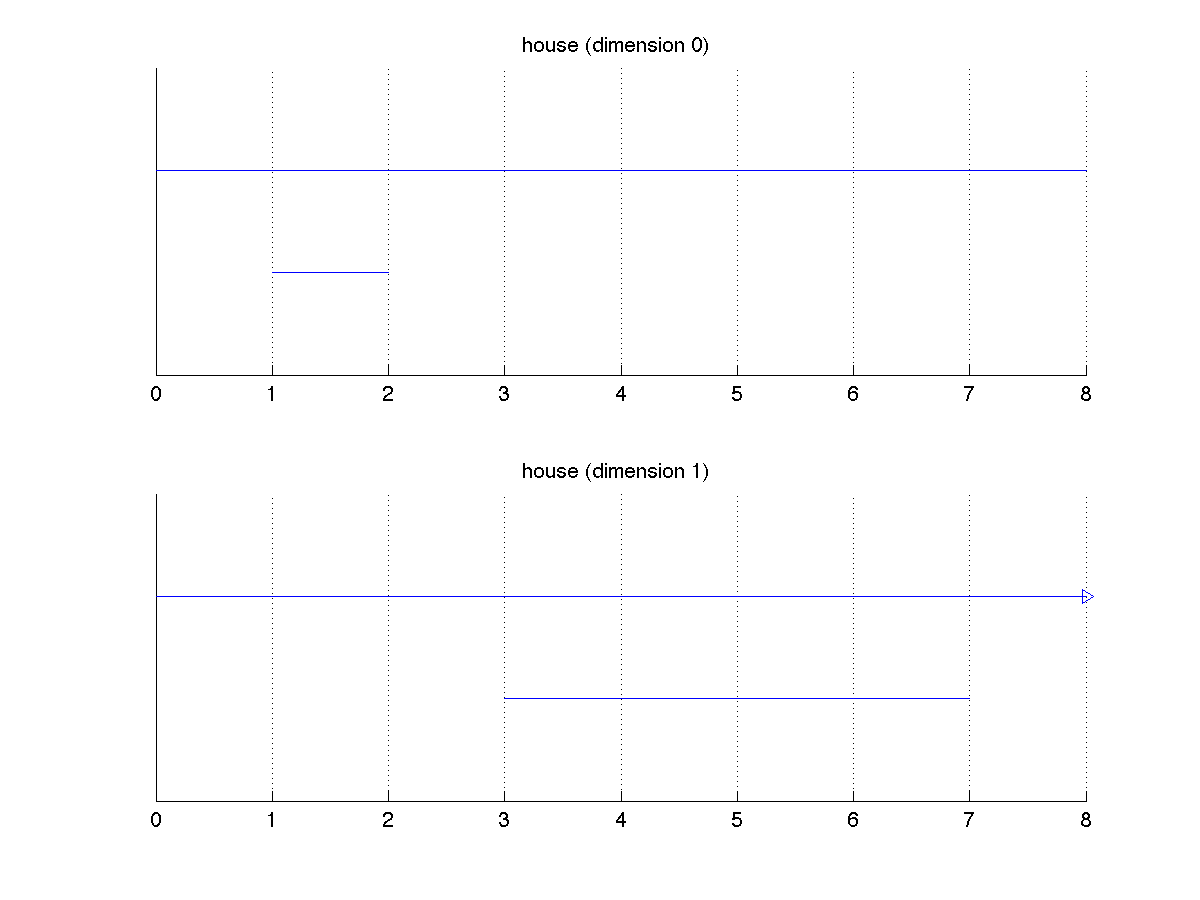
\includegraphics[width=1in]{house}
  	\end{center}
\end{wrapfigure}

Let's build a stream with nontrivial filtration times. We build a house, with the square appearing at time 0, the top vertex at time 1, the roof edges at times 2 and 3, and the roof 2-simplex at time 7.
\begin{quote} \texttt{>> stream = api.Plex4.createExplicitSimplexStream(); \\
>> stream.addVertex(1, 0); \\
>> stream.addVertex(2, 0); \\
>> stream.addVertex(3, 0); \\
>> stream.addVertex(4, 0); \\
>> stream.addVertex(5, 1); \\
>> stream.addElement([1, 2], 0); \\
>> stream.addElement([2, 3], 0); \\
>> stream.addElement([3, 4], 0); \\
>> stream.addElement([4, 1], 0); \\
>> stream.addElement([3, 5], 2); \\
>> stream.addElement([4, 5], 3); \\
>> stream.addElement([3, 4, 5], 7);
} \end{quote} % can you add more than 1 simplex at a time?
We get the default persistence computation,
\begin{quote} \texttt{>> persistence = api.Plex4.getDefaultSimplicialAlgorithm(3);
} \end{quote}
compute the intervals,
\begin{quote} \texttt{>> filtration\_index\_intervals = persistence.computeIntervals(stream);
} \end{quote}
and transform the integral intervals to floating point intervals.
\begin{quote} \texttt{>> transformer = homology.filtration.IdentityConverter.getInstance(); \\
>> filtration\_value\_intervals = transformer.transform(filtration\_index\_intervals) \\
filtration\_value\_intervals =\\
\\
Dimension: 1\newline
[3.000000, 7.000000)\newline
[0.000000, infinity)\\
\\
Dimension: 0\newline
[1.000000, 2.000000)\newline
[0.000000, infinity)\\
} \end{quote}
There are four intervals. The first is a $Betti_1$ interval, starting at filtration time 3 and ending at 7. This 1-dimensional hole is formed by the three edges of the roof. It forms when edge $[4,5]$ appears at filtration time 3 and closes when 2-simplex $[3,4,5]$ appears at filtration time 7.\\

One $Betti_0$ interval and one $Betti_1$ interval are semi-infinite. 
\begin{quote} \texttt{>> infinite\_barcodes = filtration\_value\_intervals.getInfiniteIntervals();
} \end{quote}
We can print the Betti numbers (at time 7 or infinity) as an array
\begin{quote} \texttt{>> betti\_numbers\_array = infinite\_barcodes.getBettiSequence()
} \end{quote}
\hspace{12mm}\texttt{betti\_numbers\_array =}

\hspace{19mm}$\begin{matrix}
\texttt{1}\\
\texttt{1}
\end{matrix}$
\vspace{3mm}

or as a list with entries of the form $k: Betti_k$.
\begin{quote} \texttt{>> betti\_numbers\_string = infinite\_barcodes.getBettiNumbers()\\
betti\_numbers\_string = \{0: 1, 1: 1\} \\
} \end{quote}

The method \texttt{createBarcodePlot} lets us display the intervals as a Betti barcode. The three inputs are \texttt{filtration\_value\_intervals}, a string for the filename, and the maximum filtration time (which may be adjusted $\pm 10\%$) for the plot. 
\begin{quote} \texttt{>> api.Plex4.createBarcodePlot(filtration\_value\_intervals, 'house', 8)
} \end{quote}
The files \texttt{house\_0.PNG} and \texttt{house\_1.PNG} are saved to your current directory.

\begin{figure}[htp]
  \begin{center}
    \subfigure{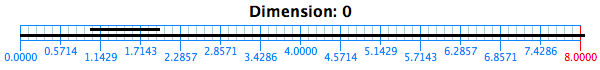
\includegraphics[width=6in]{house_0}}
    \subfigure{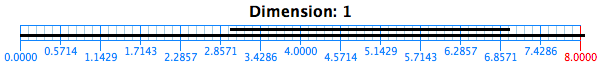
\includegraphics[width=6in]{house_1}}
   \end{center}
\end{figure}
\FloatBarrier

The filtration times are on the horizontal axis. The $Betti_k$ number of the stream at filtration time $t$ is the number of intervals in the dimension $k$ plot that intersect a vertical line through $t$. Check that the displayed intervals agree with the filtration times we built into the stream \texttt{house}. At time 0, a connected component and a 1-dimensional hole form. At time 1, a second connected component appears, which joins to the first at time 2. A second 1-dimensional hole forms at time 3, and closes at time 7. \\

%The method \texttt{Plex.scatter} displays the same information as \texttt{Plex.plot} but in a different format: an interval starting at $start$ and ending at $end$ is plotted as the point $(start,end)$ in $\mathbb{R}^2$, which is necessarily above the diagonal.
%\begin{quote} \texttt{>> Plex.scatter(intervals, 'house', 8)} \end{quote}  \index{1}{Plex.scatter}
%The produced figure is fairly large and so it is not included in this tutorial. For more information on scatter plots, see \cite{elz02}, especially Figure 7. \\




\subsection{Explicit simplex stream details}
We mention two remaining details about class ExplicitSimplexStream.\\

The methods \texttt{addElement} and \texttt{removeElementIfPresent} do not necessarily enforce the definition of a stream. They allow us to build inconsistent streams in which some simplex $\sigma \in X(t)$ contains a subsimplex $\sigma' \notin X(t)$, meaning that $X(t)$ is not a simplicial complex. The method \texttt{validateVerbose} returns \texttt{1} if our stream is consistent and returns \texttt{0} with explanation if not. 
\begin{quote} \texttt{>> stream.validateVerbose() \\
ans = 1 \\
>> stream.addElement([1, 4, 5], 0); \\
>> stream.validateVerbose() \\
Filtration index of face [4,5] exceeds that of element [1,4,5] (3 > 0) \\
Stream does not contain face [1,5] of element [1,4,5] \\
ans = 0
} \end{quote}

% Method \texttt{prune} is also sometimes useful. Command \texttt{prune($\sigma$)} removes not only simplex $\sigma$ but also any higher dimensional simplices $\tau$ containing $\sigma$. \\

%In \S \ref{sfpc} we will create SimplexStream instances that %, unlike \texttt{house}, 
%are not also ExplicitStream instances. To display or edit such streams, we will first need to use the method \texttt{makeExplicit}. See Exercise \ref{ripsExpl}. \\
% TODO

%\begin{quote} \texttt{>> house.size \\
%ans = 12 \\ 
%>> house.maxDimension \\
%ans = 2 \\




\section{Point cloud data}

A point cloud is a finite metric space, that is, a finite set of points equipped with a notion of distance. One can create a Euclidean metric space by specifying the coordinates of the points in Euclidean space, or one can create an explicit metric space by specifying all pairwise distances between points. In \S \ref{sfpc} we will learn how to build streams from point cloud data. \\

\subsection{Euclidean metric spaces}\label{euc} The Matlab script corresponding to this section is \texttt{pointcloud\_examples.m}. \\

Let's give Euclidean coordinates to the points of our house.

\vspace{-3mm}
\begin{figure}[htb]
	\centering
	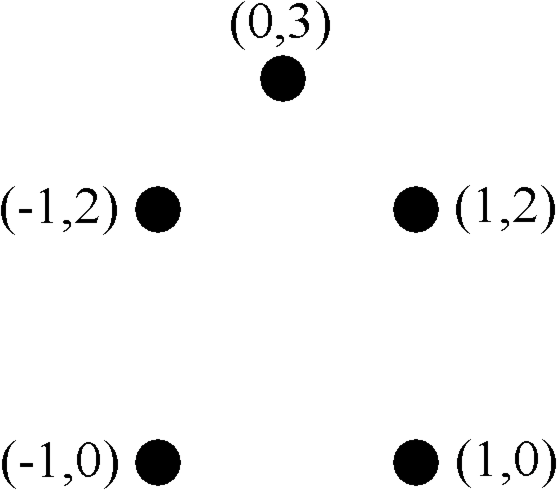
\includegraphics[width=1.55in]{houseCoord}
	\vspace{-3mm}
	\caption{The house point cloud}
	\label{fig:pdataHouse}
\end{figure}
\FloatBarrier

You can enter these coordinates manually.
\begin{quote} \texttt{>> point\_cloud = [-1,0; 1,0; 1,2; -1,2; 0,3]} \end{quote}
\hspace{12mm}\texttt{point\_cloud =}

\hspace{19mm}$\begin{matrix}
\texttt{-1} && \texttt{0}\\
\texttt{ 1} && \texttt{0}\\
\texttt{ 1} && \texttt{2}\\
\texttt{-1} && \texttt{2}\\
\texttt{ 0} && \texttt{3}\\
\end{matrix}$
\vspace{3mm}

Or, these coordinates are stored as a JavaPlex example.
\begin{quote} \texttt{>> point\_cloud = examples.PointCloudExamples.getHouseExample();\\} \end{quote}
% TODO: Need to change the ordering of these points in the source code to be consistent with the ordering in the house figure and in the previous tutorial

We create a metric space using these coordinates. The input to the EuclideanMetricSpace method is a matrix whose $i$-th row lists the coordinates of the $i$-th point.
\begin{quote} \texttt{>> m\_space = metric.impl.EuclideanMetricSpace(point\_cloud);} \end{quote}
We can return the coordinates of a specific point. Note the points are indexed starting at 0.
\begin{quote} \texttt{>> m\_space.getPoint(0)} \end{quote}
\hspace{12mm}\texttt{ans =}

\hspace{19mm}$\begin{matrix}
\texttt{-1}\\
\texttt{ 0}
\end{matrix}$

\begin{quote} \texttt{>> m\_space.getPoint(2)} \end{quote}
\hspace{12mm}\texttt{ans =}

\hspace{19mm}$\begin{matrix}
\texttt{ 1}\\
\texttt{ 2}
\end{matrix}$

A metric space can return the distance between any two points.
\begin{quote} \texttt{>> m\_space.distance(m\_space.getPoint(0), m\_space.getPoint(2))\\
ans = 2.8284\\
} \end{quote}
%The method \texttt{dimension} returns the dimension of the Euclidean space containing our points.
%\begin{quote} \texttt{>> pdataHouse.dimension \index{1}{dimension}\\
%ans = 2
%} \end{quote}
%The method \texttt{coordinate($i$,$j$)} returns the $j$-th coordinate of point $i$. Points are indexed starting at one but coordinates are indexed starting at zero. We display the coordinates of point 5.
%\begin{quote} \texttt{>> pdataHouse.coordinate(5, 0) \index{1}{coordinate}\\
%ans = 0 \\
%>> pdataHouse.coordinate(5, 1) \\
%ans = 3 \\
%} \end{quote}
%We can display all of point 5 at once. The first command creates a vector \texttt{vec} of length \texttt{dimension}, and the second command writes point 5 to \texttt{vec}.
%\begin{quote} \texttt{>> vec = zeros(2, 1); \\
%>> pdataHouse.get\_pt(5, vec) \\
%ans  = }\end{quote}
% vec is still [0,0], however. Weird!

%\hspace{15mm} \texttt{0}

%\hspace{15mm} \texttt{3}

{\em Figure 8 example.} We select 100 points randomly from a figure eight, that is, the union of unit circles centered at (0,1) and (0,-1).
\begin{quote} \texttt{>> point\_cloud = examples.PointCloudExamples.getRandomFigure8Points(100);
} \end{quote}
We plot the points.
\begin{quote} \texttt{>> figure\\
>> plot(point\_cloud(:,1), point\_cloud(:,2), '.')\\
>> axis equal\\
} \end{quote}

{\em Torus example.} We select 2000 points randomly from a torus in $\mathbb{R}^3$ with inner radius 1 and outer radius 2. The first input is the number of points, the second input is the inner radius, and the third input is the outer radius
\begin{quote} \texttt{>> point\_cloud = examples.PointCloudExamples.getRandomTorusPoints(2000, 1, 2);
} \end{quote}
We plot the points.
\begin{quote} \texttt{>> figure\\
>> plot3(point\_cloud(:,1), point\_cloud(:,2), point\_cloud(:,3), '.')\\
>> axis equal\\
} \end{quote}

{\em Sphere product example.} We select 1000 points randomly from the unit torus $S^1 \times S^1$ in $\mathbb{R}^4$. The first input is the number of points, the second input is the dimension of each sphere, and the third input is the number of sphere factors.
\begin{quote} \texttt{>> point\_cloud = examples.PointCloudExamples.getRandomTorusPoints(1000, 1, 2);
} \end{quote}
Plotting the third and fourth coordinates of each point gives a circle $S^1$.
\begin{quote} \texttt{>> figure\\
>> plot(point\_cloud(:,3), point\_cloud(:,4), '.')\\
>> axis equal\\
} \end{quote}




\subsection{Explicit metric spaces}
We can also create a metric space from a distance matrix using the command \texttt{ExplicitMetricSpace}. For a point cloud in Euclidean space, this method is generally less convenient than the command \texttt{EuclideanMetricSpace}. However, command \texttt{ExplicitMetricSpace} can be used for a point cloud in an arbitrary (perhaps non-Euclidean) metric space. \\

The Matlab script corresponding to this section is \texttt{explicit\_metric\_space.m}. \\

The matrix \texttt{distances} summarizes the metric for our house points in Figure \ref{fig:pdataHouse}: entry $(i,j)$ is the distance from point $i$ to point $j$.
%Don't forget you can copy and paste commands from \texttt{commandListMatlab.rtf} into the Matlab window, or enter them using a script! 

\hspace{8mm}\texttt{>> distances = [0,2,sqrt(8),2,sqrt(10);}

\hspace{15mm}\texttt{2,0,2,sqrt(8),sqrt(10);}

\hspace{15mm}\texttt{sqrt(8),2,0,2,sqrt(2);}

\hspace{15mm}\texttt{2,sqrt(8),2,0,sqrt(2);}

\hspace{15mm}\texttt{sqrt(10),sqrt(10),sqrt(2),sqrt(2),0]}

\vspace{5mm}
\hspace{8mm}\texttt{distances =}\\

\hspace{15mm}$\begin{matrix}
\texttt{0} & \texttt{2.0000} & \texttt{2.8284} & \texttt{2.0000} & \texttt{3.1623}\\
\texttt{2.0000} & \texttt{0} & \texttt{2.0000} & \texttt{2.8284} & \texttt{3.1623}\\
\texttt{2.8284} & \texttt{2.0000} & \texttt{0} & \texttt{2.0000} & \texttt{1.4142}\\
\texttt{2.0000} & \texttt{2.8482} & \texttt{2.0000} & \texttt{0} & \texttt{1.4142}\\
\texttt{3.1623} & \texttt{3.1623} & \texttt{1.4142} & \texttt{1.4142} & \texttt{0}
\end{matrix}$
\vspace{3mm}

We create a metric space from this matrix. 
\begin{quote} \texttt{>> m\_space = metric.impl.ExplicitMetricSpace(distances);
} \end{quote}
We return the distance between points 0 and 2.
\begin{quote} \texttt{>> m\_space.distance(m\_space.getPoint(0), m\_space.getPoint(2))\\
ans = 2.8284\\
} \end{quote}

% Be careful: the constructor \texttt{DistanceData()} will accept matrices that fail to be symmetric, square, or nonnegative, creating ``metrics'' that do not satisfy the mathematical definiton. The triangle inequality is similarly easy to ignore. However, asking for the distance between a point and itself will always return zero, even if you input a distance matrix with non-zero diagonal entries. \\

%\subsection{Subclass Torus}
%The following command constructs a $20 \times 20$ grid of points on the 2 dimensional unit torus.
%\begin{quote} \texttt{>> tor20 = Plex.Torus(20, 2);} \end{quote}
%The methods of \S \ref{euc}, except for \texttt{coordinate} and \texttt{get\_pt}, work as well with \texttt{tor20}. Method \texttt{dimension} now returns the dimension of the torus manifold. We will use \texttt{tor20} shortly. \\




\section{Streams from point cloud data}\label{sfpc}

In \S \ref{streams} we built instances of the class SimplexStream from scratch. In this section we construct streams from a point cloud $Z$. We use the three subclasses RipsStream, WitnessStream, and LazyWitnessStream, which build the Vietoris-Rips, witness, and lazy witness streams. See \cite{dsc04} for additional information. \\

All three subclasses take four of the same inputs: the granularity $\delta$, the maximum dimension $d_{max}$, the maximum filtration time $t_{max}$, and a point cloud $Z$ stored as a PointData instance. The first three inputs allow the user to limit the size of the constructed stream, for computational efficiency. No simplices above dimension $d_{max}$ are included. The persistent homology of the resulting stream can be calculated only up to dimension $d_{max}-1$ (do you see why?). Also, instead of computing complex $X(t)$ for all $t \geq 0$, we only compute $X(t)$ for $t = 0, \delta$, $2\delta$, $3\delta$, ..., $N\delta$, where $N$ is the largest integer such that $N\delta \leq t_{max}$. In this tutorial we use $\delta = 0.001$. \\

When working with a new dataset, don't choose $d_{max}$ and $t_{max}$ too large initially. First get a feel for how fast the complexes are growing, and then raise $d_{max}$ and $t_{max}$ nearer to the computational limits. If you ever choose $d_{max}$ or $t_{max}$ too large and Matlab seems to be running forever, pressing the ``control'' and ``c'' buttons simultaneously sometimes halts the computation. \\

I am currently working with Jan Segert on interactive visualizations of the Rips and Witness filtrations for the Wolfram Demonstrations Project. We have preliminary drafts of the demonstrations. Please email me if you'd like to check them out; in particular, the witness filtrations can be hard to visualize.




\subsection{Subclass RipsStream}\label{ripsStream}
Let  $d(\ \cdot\ ,\ \cdot \ )$ denote the distance between two points. A natural stream to build is the Rips stream. The complex Rips$(Z,t)$ is defined as follows: 
\begin{itemize}
\item{the vertex set is $Z$.}
\item{for vertices $a$ and $b$, edge $[ab]$ is in Rips$(Z,t)$ if $d(a,b) \leq t$.}
\item{a higher dimensional simplex is in Rips$(Z,t)$ if all of its edges are.}
\end{itemize}
Note that $\mbox{Rips}(Z,t) \subset \mbox{Rips}(Z,s)$ whenever $t\leq s$, so the Rips stream is a filtered simplicial complex. Since a Rips complex is the maximal simplicial complex that can be built on top of its 1-skeleton, it is a {\em flag complex}. \\

Let's build a Rips stream instance \texttt{ripsHouse} from the PointData instance \texttt{pdataHouse}. Note this stream is different than the ExplicitStream \texttt{house} we built in \S \ref{explicitStream}.
\begin{quote} \texttt{>> ripsHouse = Plex.RipsStream(0.001, 3, 4, pdataHouse);} \end{quote} \index{1}{Plex.RipsStream}
The order of the inputs is \texttt{RipsStream(}$\delta,\ d_{max},\ t_{max},\ Z$\texttt{)}. Since $d_{max} = 3$ we can compute up to second dimensional persistent homology. For a Rips stream, the parameter $t_{max}$ is the maximum possible edge length. Since $t_{max} = 4$ is greater than the diameter ($\sqrt{10}$) of our point cloud, all edges will eventually form. \\

We compute and display the Betti intervals. Typically the last input for the method \texttt{Plex.plot} will be $t_{max}$, since there is no reason to display filtration times that we haven't computed.
\begin{quote} \texttt{>> intervals = Plex.Persistence.computeIntervals(ripsHouse); \index{1}{Plex.Persistence.computeIntervals}\\
>> Plex.plot(intervals, 'ripsHouse', 4) \index{1}{Plex.plot}
} \end{quote}

\begin{figure}[htp]
  \begin{center}
    \subfigure{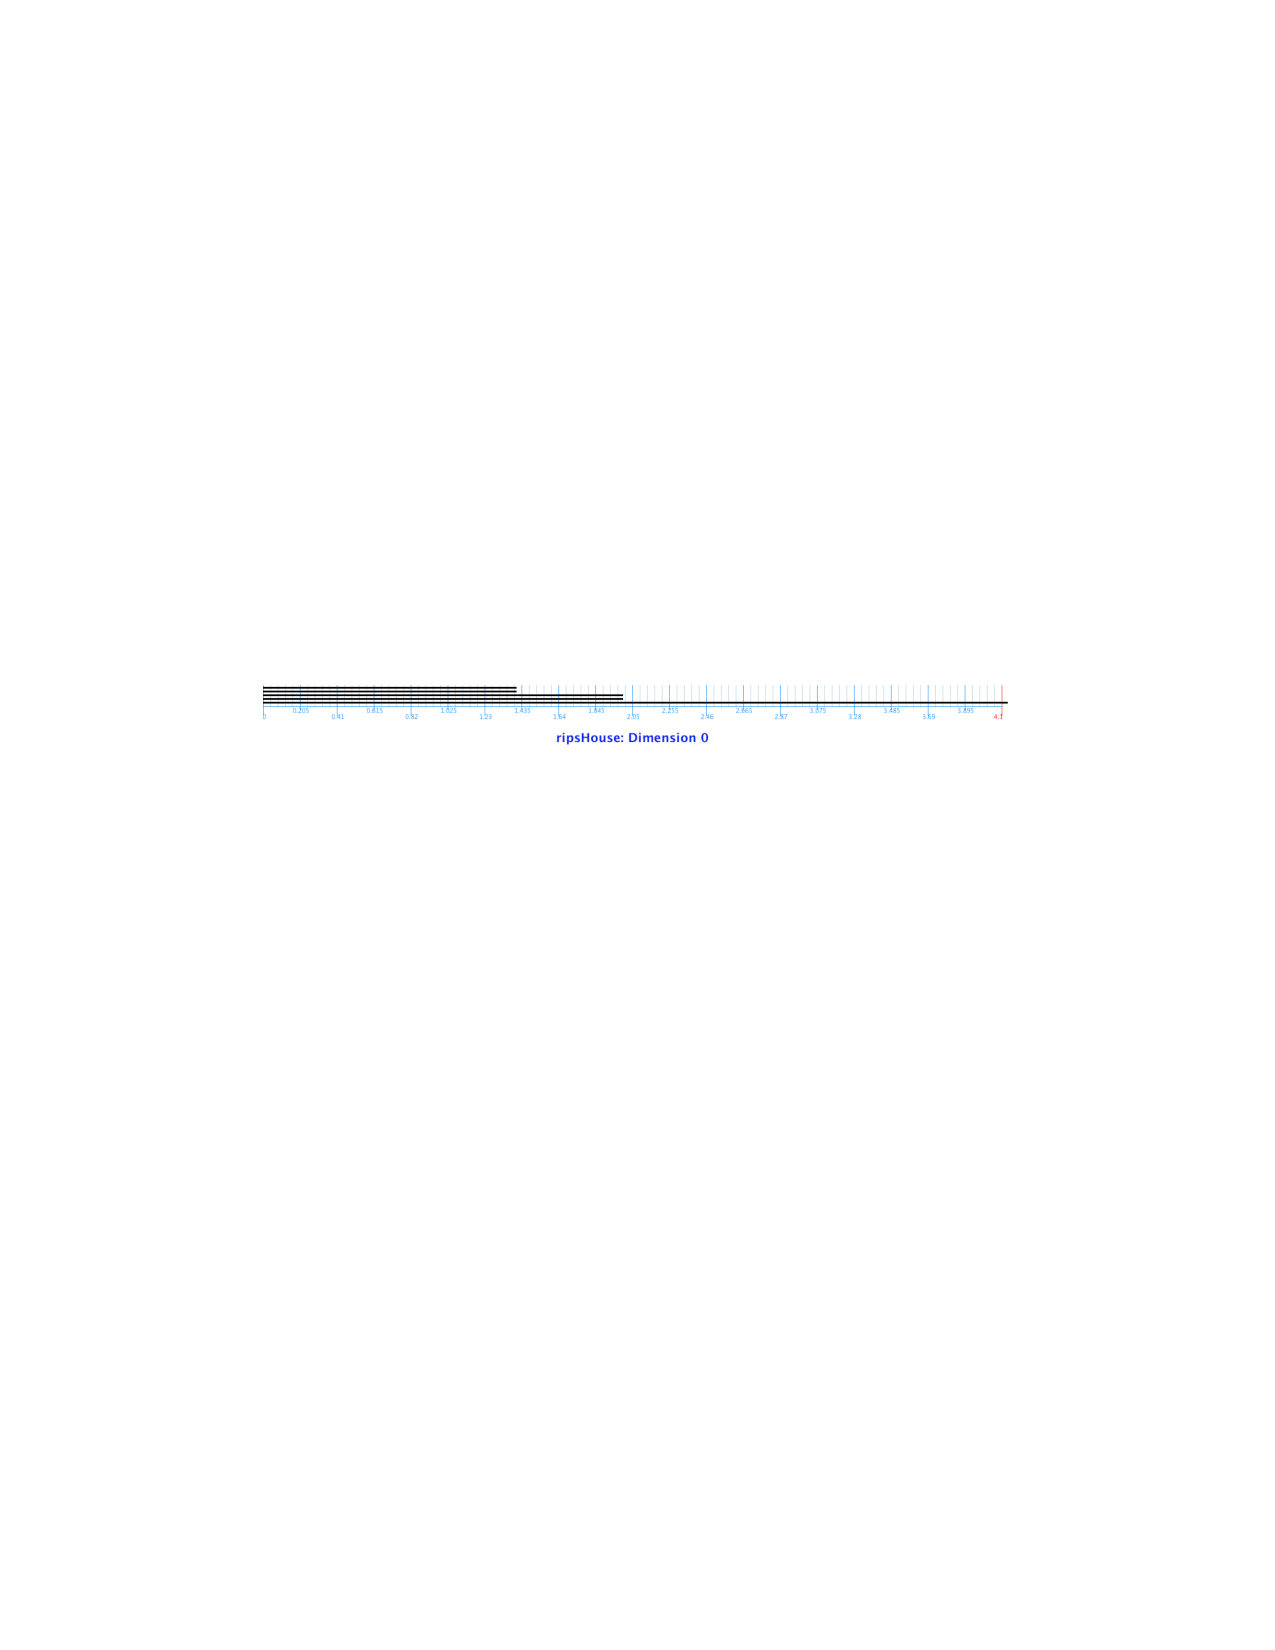
\includegraphics[width=6in]{ripsHouse0}}
    \subfigure{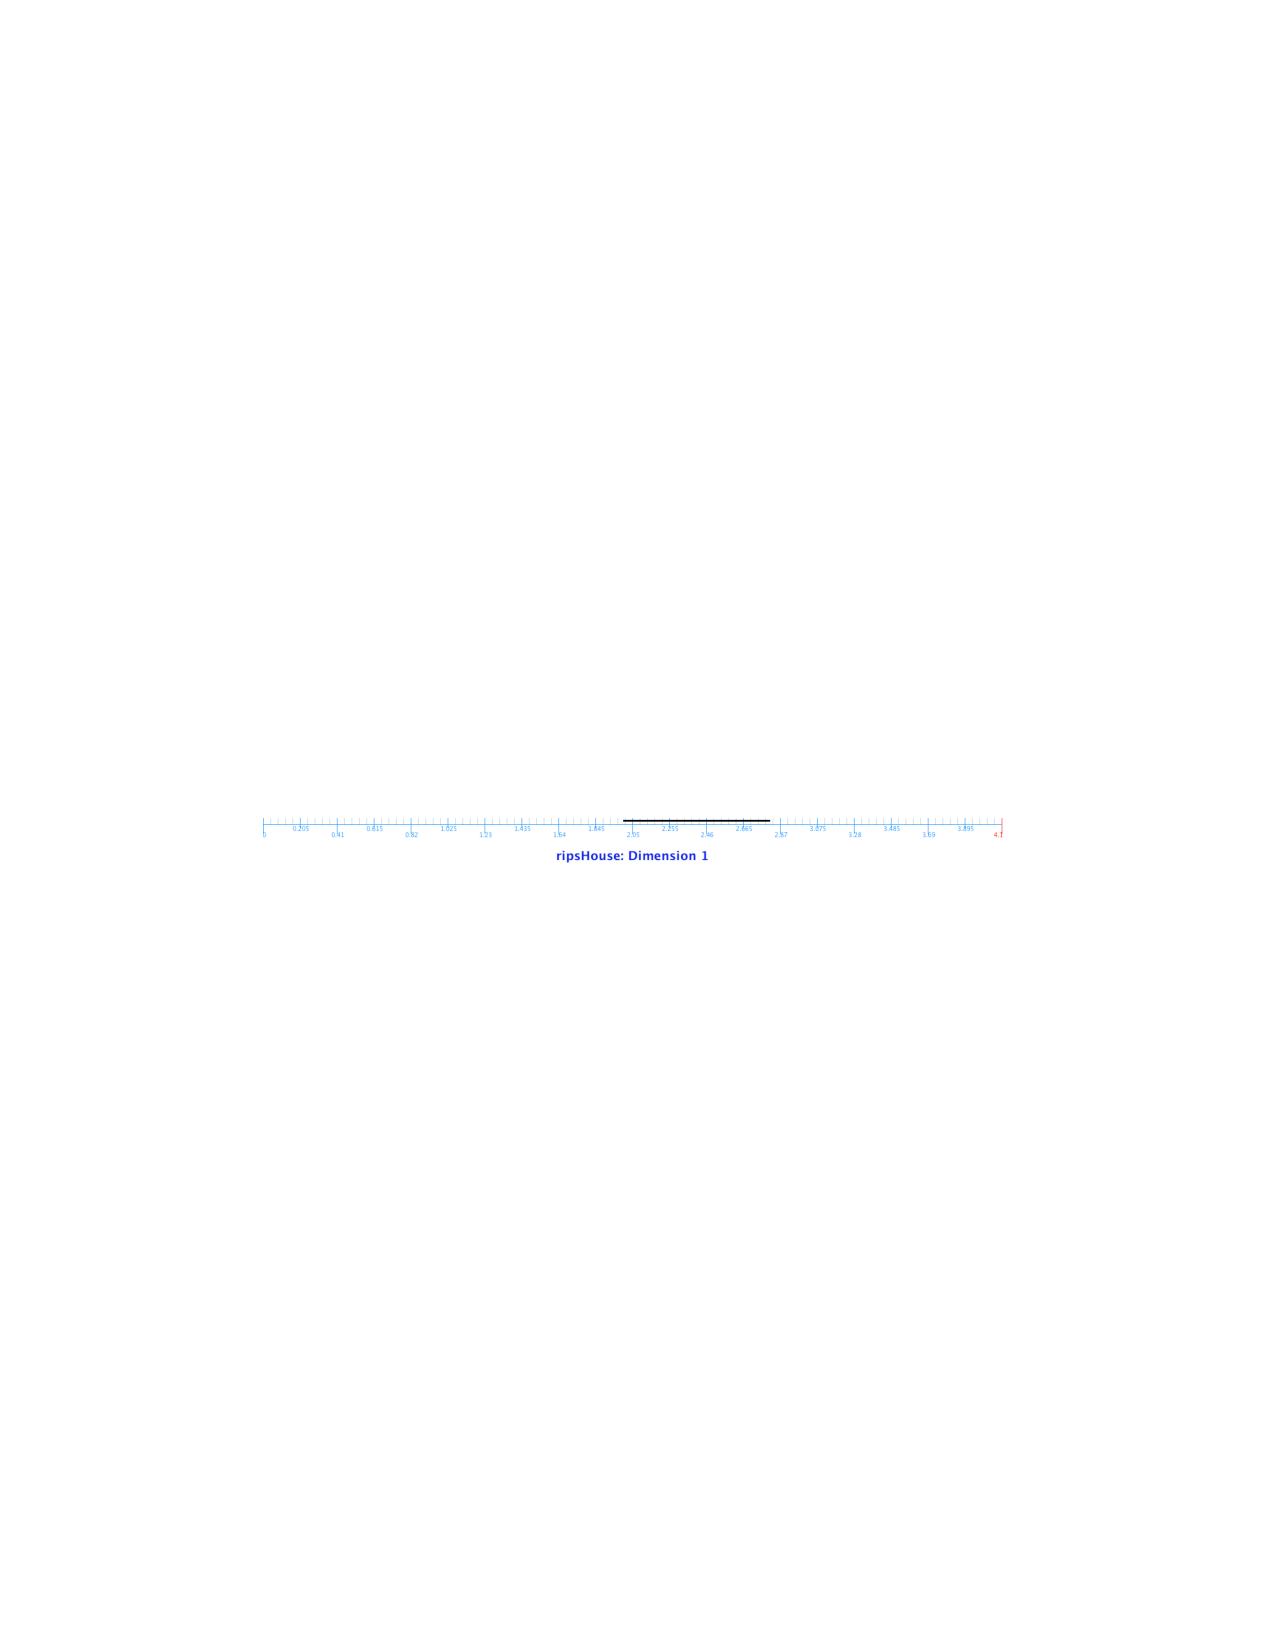
\includegraphics[width=6in]{ripsHouse1}}
   \end{center}
\end{figure}
\FloatBarrier

The second dimensional Betti plot does not appear because there are no $Betti_2$ intervals. Check that these plots are consistent with the Rips definition: edges $[3,5]$ and $[4,5]$ appear at filtration time $t = \sqrt{2}$; the square appears at $t = 2$; the square closes at $t = \sqrt{8}$. \\

\begin{exercise}\label{ripsExpl}
Change \texttt{ripsHouse} into an explicit stream
\begin{quote} \texttt{>> ripsExpl = Plex.makeExplicit(ripsHouse);} \end{quote} \index{1}{Plex.makeExplicit}
Check that you can display and edit stream \texttt{ripsExpl} using the methods of \S \ref{streams}. \\
\end{exercise}

{\em Torus example.} Try the following sequence of commands. We select a $20 \times 20$ grid of noisy points from a torus and build the RipsStream \texttt{ripsT20}. The fourth command returns the total number of simplices in \texttt{ripsT20}.
\begin{quote} \texttt{>> pointsT20 = pointsTorus(20); \index{1}{pointsTorus.m}\\
>> pdataT20 = EuclideanArrayData(pointsT20); \index{1}{EuclideanArrayData}\\
>> ripsT20 = Plex.RipsStream(0.001, 3, 0.9, pdataT20); \index{1}{Plex.RipsStream}\\
>> ripsT20.size \index{1}{size}\\
ans = 82831\hspace{30mm} \% Generally close to 80000 \\
>> intervals = Plex.Persistence.computeIntervals(ripsT20); \index{1}{Plex.Persistence.computeIntervals}\\
>> Plex.FilterInfinite(intervals) \index{1}{FilterInfinite}\\
ans = BN\{1, 2, 1\} \\
>> Plex.plot(intervals, 'ripsT20', 0.9) \index{1}{Plex.plot}\\
} \end{quote}

We do not include the Betti intrervals because the plots are very tall. The diameter of this torus (before adding noise) is $\sqrt{8}$, so choosing $t_{max} = 0.9$ likely will not show all homological activity. However, the torus will be reasonably connected by this time. Note the semi-infinite intervals match the correct numbers $Betti_0 = 1$, $Betti_1 = 2$, $Betti_2 = 1$ for a torus. \\

This example makes it clear that the computed ``semi-infinite'' intervals do not necessarily persist until $t = \infty$: in a Rips stream, once $t$ is greater than the diameter of the point cloud, the Betti numbers for Rips$(Z,t)$ will be $ Betti_0 = 1$, $Betti_1 = Betti_2 = ... = 0$. The computed semi-infinite intervals are merely those that persist until $t = t_{max}$. \\ %(or, to be precise, until $t = N\delta$ where $N$ is the largest integer such that $N\delta \leq t_{max}$).\\

\begin{exercise}
Slowly increase the values for $t_{max}$, $d_{max}$, or the grid length (20 above) and note how quickly \texttt{ripsT20.size} and the computation time grows. Separately increasing $t_{max}$ from 0.9 to 1, $d_{max}$ from 3 to 4, or the grid length from 20 to 22 each roughly doubles \texttt{ripsT20.size}. \\
\end{exercise}

\begin{exercise}
Find a planar dataset $Z$ and a filtration value $t$ such that $Betti_2(\mbox{Rips}(Z,t))\neq0$. Build a RipsStream to confirm your answer. \\
\end{exercise}

\begin{exercise}
Find a planar dataset $Z$ and a filtration value $t$ such that $Betti_{6}(\mbox{Rips}(Z,t))\neq0$. When building a RipsStream to confirm your answer, don't forget to choose $d_{max} = 7$. \\
\end{exercise}




\subsection{Landmark selection}\label{lands}
For larger datasets, if we include every data point as a vertex, as in the Rips construction, our streams will quickly contain too many simplices for efficient computation. The witness stream and the lazy witness stream address this problem. In building these streams, we select a subset $L \subset Z$, called landmark points, as the only vertices. All data points in $Z$ help serve as witnesses for the inclusion of higher dimensional simplices. \\

There are two common methods for selecting landmark points. The first is to choose the landmarks $L$ randomly from point cloud $Z$. We select 25 random landmarks from figure eight PointData instance \texttt{pdataF100}.
\begin{quote} \texttt{>> L1 = WitnessStream.makeRandomLandmarks(pdataF100, 25); \index{1}{WitnessStream.makeRandomLandmarks}\\
>> length(L1) \index{1}{length}\\
ans = 26
} \end{quote}
Vector \texttt{L} always has first entry zero. The remaining 25 entries contain the indices of the random landmark vertices. \\

The second method for selecting landmark points, called sequential maxmin, is a greedy inductive selection process. Pick the first landmark randomly from $Z$. Inductively, if $L_{i-1}$ is the set of the first $i-1$ landmarks, then let the $i$-th landmark be the point of $Z$ which maximizes the function $z \mapsto d(z,L_{i-1})$, where $d(\ \cdot\ ,\ \cdot\ )$ is the distance between the point and the set. \\

Landmarks chosen using sequential maxmin tend to cover the dataset and to be spread apart from each other. A disadvantage is that outlier points tend to be selected. Sequential maxmin landmarks are used in \cite{ac09} and \cite{cidsz08}. \\

JavaPlex does not yet have a command for sequential maxmin landmark selection, so we use the m-file \texttt{maxminLandmarks.m}. The first input is a matrix and the second input is the number of landmarks to be selected. The third input is either the character \texttt{'e'} or \texttt{'d'}. Use \texttt{'e'} in the EuclideanArrayData case where the first input should be interpreted as an $N \times n$ matrix of $N$ points in $\mathbb{R}^n$. Use \texttt{'d'} in the DistanceData case where the first input should be interpreted as an $N \times N$ distance matrix for $N$ points in an arbitrary metric space. \\

{\em Case EuclideanArrayData.} Recall the figure eight example.
\begin{quote} \texttt{>> pdataF100 = EuclideanArrayData(pointsF100); \index{1}{EuclideanArrayData}
} \end{quote}
We select 25 sequential maxmin landmarks.
\begin{quote} \texttt{>> L2 = maxminLandmarks(pointsF100, 25, 'e'); \index{1}{maxminLandmarks.m}\\
} \end{quote}

Plot landmark points \texttt{L1} and \texttt{L2} to see the difference between random and sequential maxmin landmark selection.

\begin{quote} \texttt{>> pointsL1 = pointsF100(L1(2:end),:); \\
>> plot(pointsL1(:,1), pointsL1(:,2), 'o'), axis equal \index{1}{plot}\\
>> pointsL2 = pointsF100(L2(2:end),:); \\
>> figure; \quad \% This makes our next plot appear in a new window \index{1}{figure}\\
>> plot(pointsL2(:,1), pointsL2(:,2), 'o'), axis equal
} \end{quote}

\begin{figure}[htp]
  \begin{center}
  \addtocounter{figure}{1} 
  \setcounter{subfigure}{0} % so that the figures are (a), (b) and not (c), (d)
    \subfigure[Random landmarks]{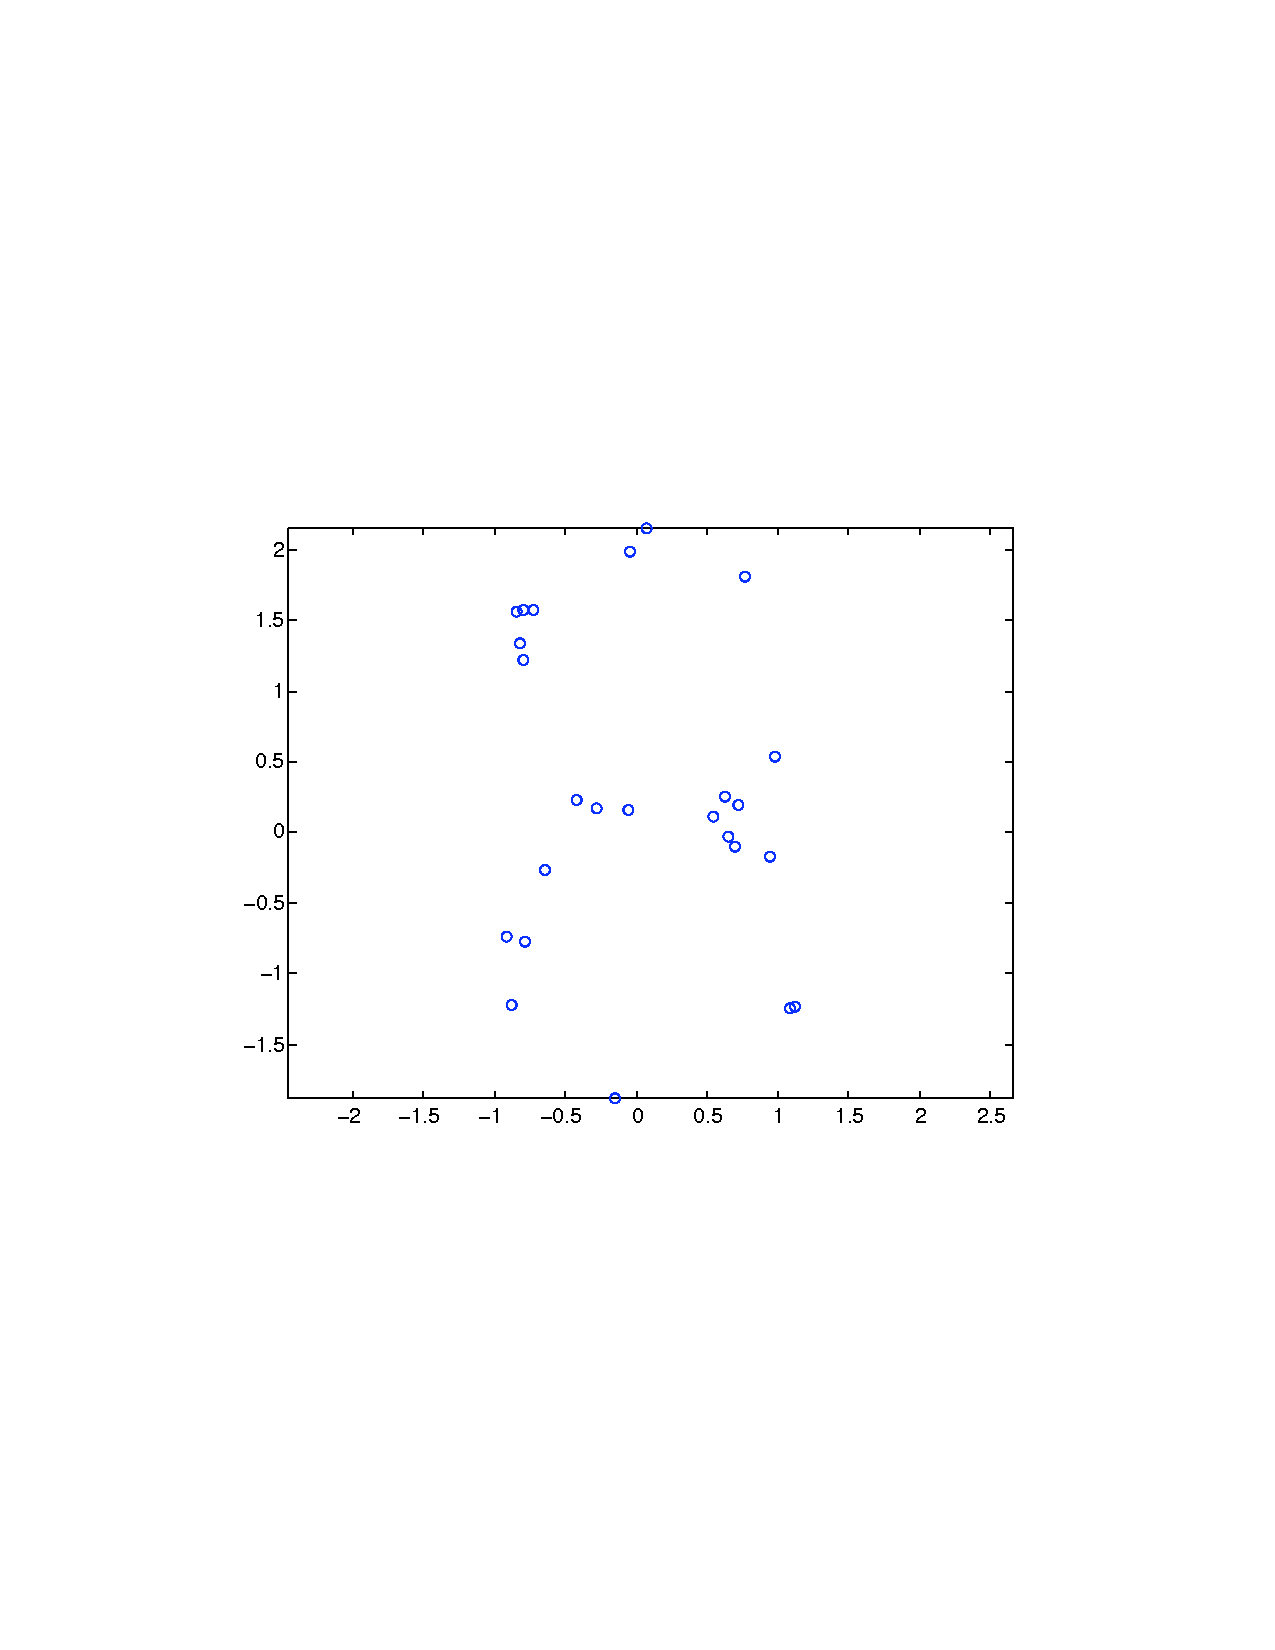
\includegraphics[width=3in]{fig8landsRand}} \label{counterPurposes}
    \subfigure[Sequential maxmin]{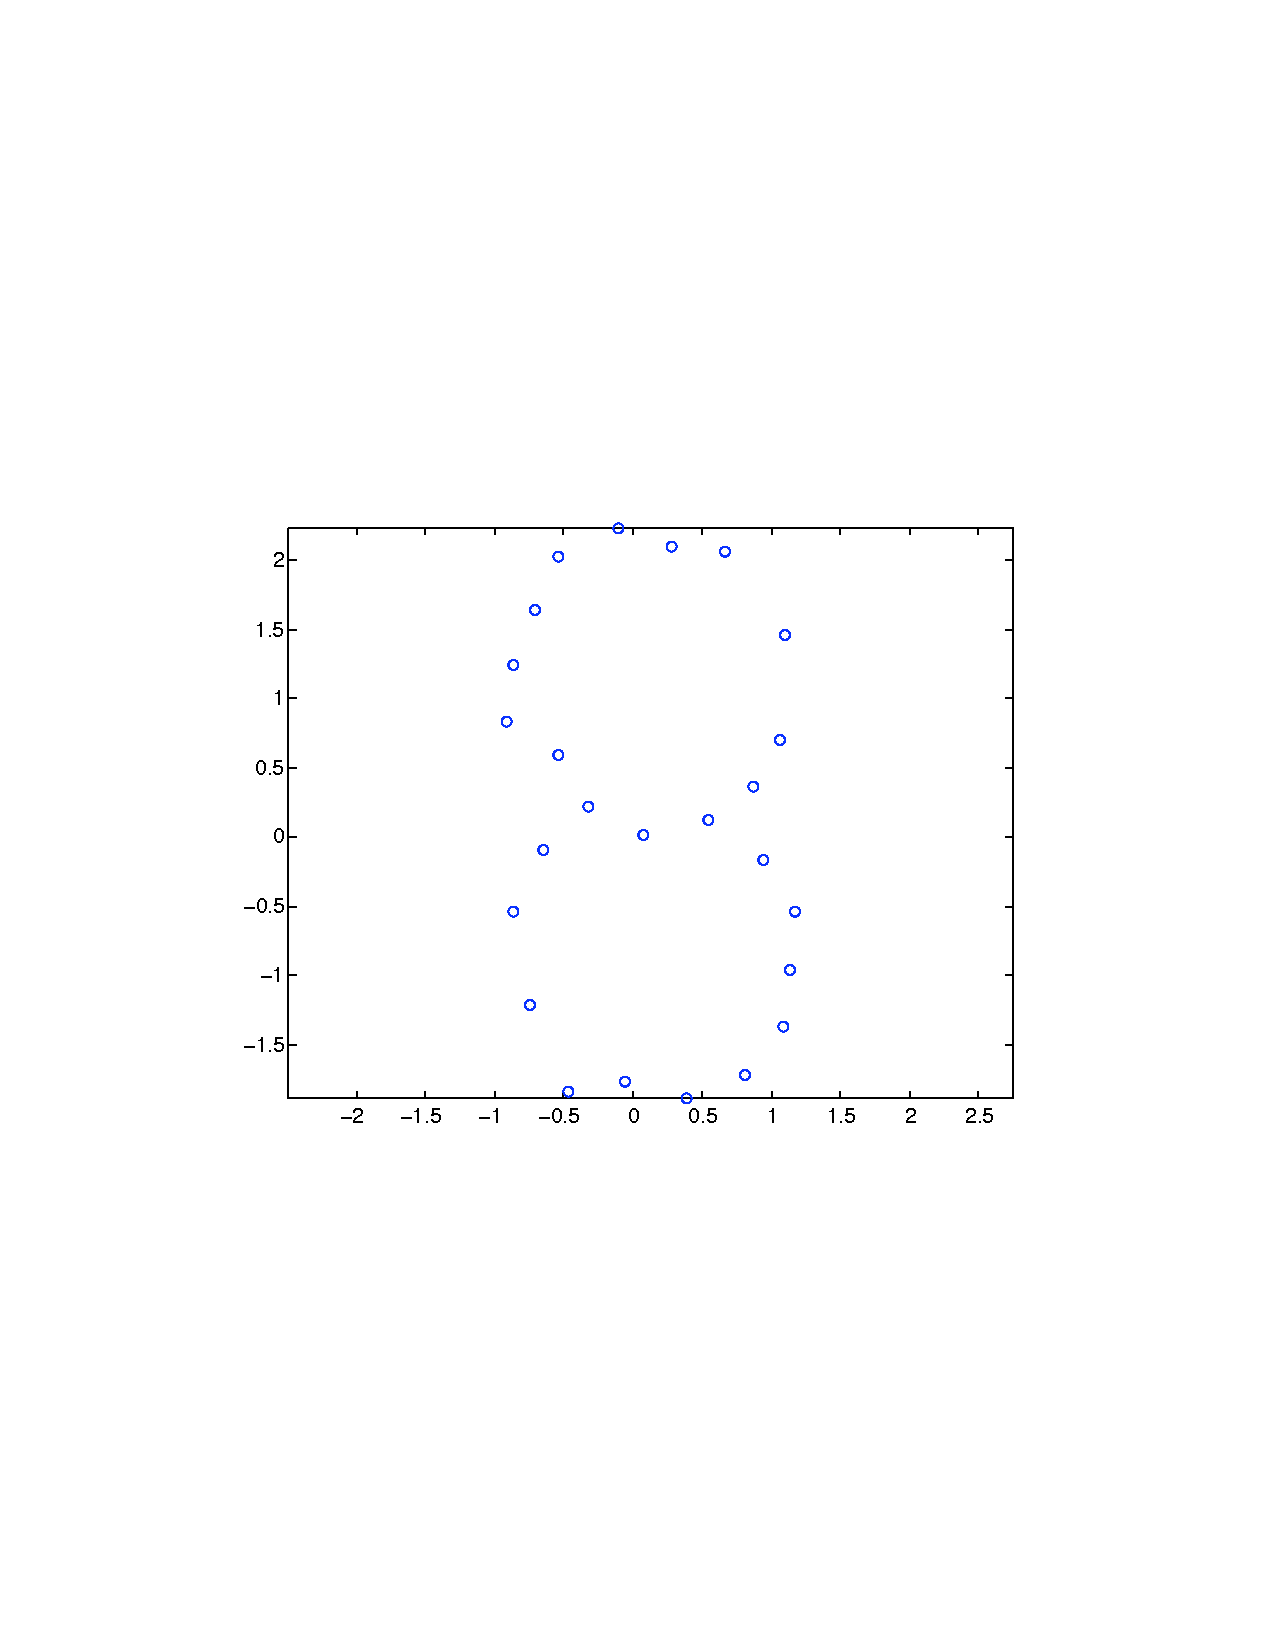
\includegraphics[width=3in]{fig8landsMaxmin}}
   \end{center}
\end{figure}

Sequential maxmin seems to do a better job of choosing landmarks that cover the figure eight and that are spread apart. \\

{\em Case DistanceData.} Recall the house example.
\begin{quote} \texttt{>> pdataHouseDD = DistanceData(distances); \index{1}{DistanceData}
} \end{quote}
We select 3 sequential maxmin landmarks.
\begin{quote} \texttt{>> L = maxminLandmarks(distances, 3, 'd') \index{1}{maxminLandmarks.m}\\
L =
} \end{quote}

\hspace{15mm} \texttt{0}

\hspace{15mm} \texttt{3}

\hspace{15mm} \texttt{1}

\hspace{15mm} \texttt{2} \\

Given point cloud $Z$ and landmark subset $L$, we define $\texttt{R} = \max_{z\in Z}\bigl\{d(z,L)\bigr\}$. Number \texttt{R} reflects how finely the landmarks cover the dataset. We often use it as a guide for selecting the maximum filtration value $t_{max}$ for a WitnessStream or LazyWitnessStream instance. \\

\begin{exercise}
Let $Z$ be the point cloud in Figure \ref{fig:pdataHouse} from \S \ref{euc}, corresponding to PointData instance \texttt{pdataHouse}. Suppose we are using sequential maxmin to select a set $L$ of 3 landmarks, and the first (randomly selected) landmark is $(1,0)$. Find by hand the other two landmarks in $L$. \\
\end{exercise}

\begin{exercise}
Let $Z$ be a point cloud and $L$ a landmark subset. Show that if $L$ is chosen via sequential maxmin, then for any $l_i,l_j\in L$, we have $d(l_i,l_j)\geq\texttt{R}$. \\
\end{exercise}




\subsection{Subclass WitnessStream}
Suppose we are given a point cloud $Z$ and landmark subset $L$. Let $m_k(z)$ be the distance from a point $z \in Z$ to its $(k+1)$-th closest landmark point. The witness stream complex $W(Z,L,t)$ is defined as follows.
\begin{itemize}
\item{the vertex set is $L$.}
\item{for $k>0$ and vertices $l_i$, the $k$-simplex $[l_0 l_1 ... l_k]$ is in $W(Z,L,t)$ if all of its faces are, and if there exists a witness point $z \in Z$ such that $\max\bigl\{d(l_0,z), d(l_1,z), ..., d(l_k,z)\bigr\} \leq t+m_k(z)$. }
\end{itemize}
Note that $W(Z,L,t) \subset W(Z,L,s)$ whenever $t\leq s$. Note that a landmark point can serve as a witness point. \\

\begin{exercise}
Let $Z$ be the point cloud in Figure \ref{fig:pdataHouse} from \S \ref{euc}, corresponding to PointData instance \texttt{pdataHouse}. Let $L = \{(1,0),(0,3),(-1,0)\}$ be the landmark subset. Find by hand the filtration time for the edge between vertices $(1,0)$ and $(0,3)$. Which point or points witness this edge? What is the filtration time for the lone 2-simplex $[(1,0),(0,3),(-1,0)]$? \\
\end{exercise}

{\em Torus example.} Let's build a WitnessStream instance for $100^2$ points from a noisy torus, with 50 random landmarks. The fourth command returns the landmark covering measure \texttt{R} from \S \ref{lands}. The fifth command returns our witness stream. The order of inputs is \texttt{WitnessStream(}$\delta,\ d_{max},\ t_{max},\ L,\ Z$\texttt{)}. Often the value for $t_{max}$ is chosen in proportion to \texttt{R}.
\begin{quote} \texttt{>> pointsT100 = pointsTorus(100); \index{1}{pointsTorus.m}\\
>> pdataT100 = EuclideanArrayData(pointsT100);\index{1}{EuclideanArrayData}\\
>> L = WitnessStream.makeRandomLandmarks(pdataT100, 50); \index{1}{WitnessStream.makeRandomLandmarks}\\
>> R = WitnessStream.estimateRmax(pdataT100, L) \index{1}{WitnessStream.estimateRmax}\\
R = 1.3188 \hspace{28mm} \% Generally close to 1.2 \\
>> witT100 = Plex.WitnessStream(0.001, 3, R/8, L, pdataT100); \index{1}{Plex.WitnessStream}\\ % R/8 since R/4 is getting slow.
>> witT100.size \index{1}{size}\\
ans = 3320\hspace{30mm} \% Generally close to 3000
} \end{quote}


We plot the Betti intervals.
\begin{quote} \texttt{>> intervals = Plex.Persistence.computeIntervals(witT100); \index{1}{Plex.Persistence.computeIntervals}\\
>> Plex.plot(intervals, 'witT100', R/8)} \end{quote} \index{1}{Plex.plot}

\begin{figure}[htp]
  \begin{center}
    \subfigure{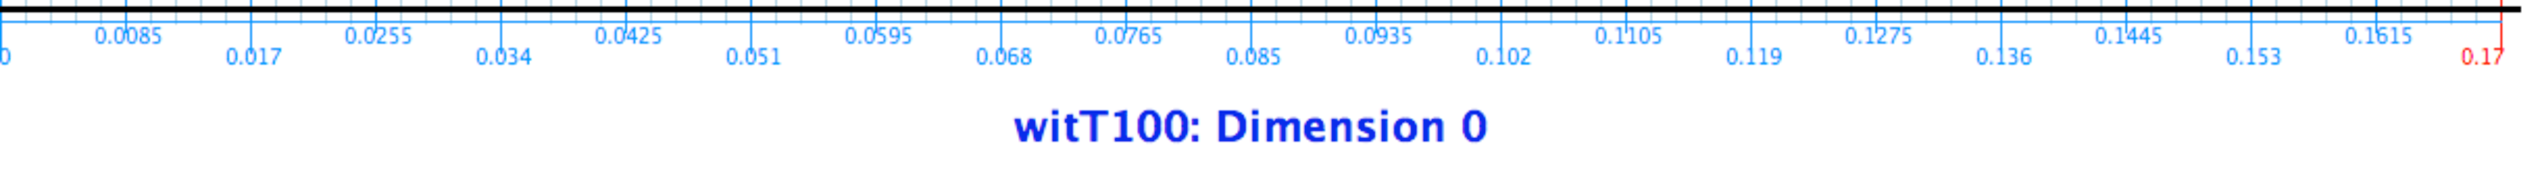
\includegraphics[width=6in]{witT100_0}}
    \subfigure{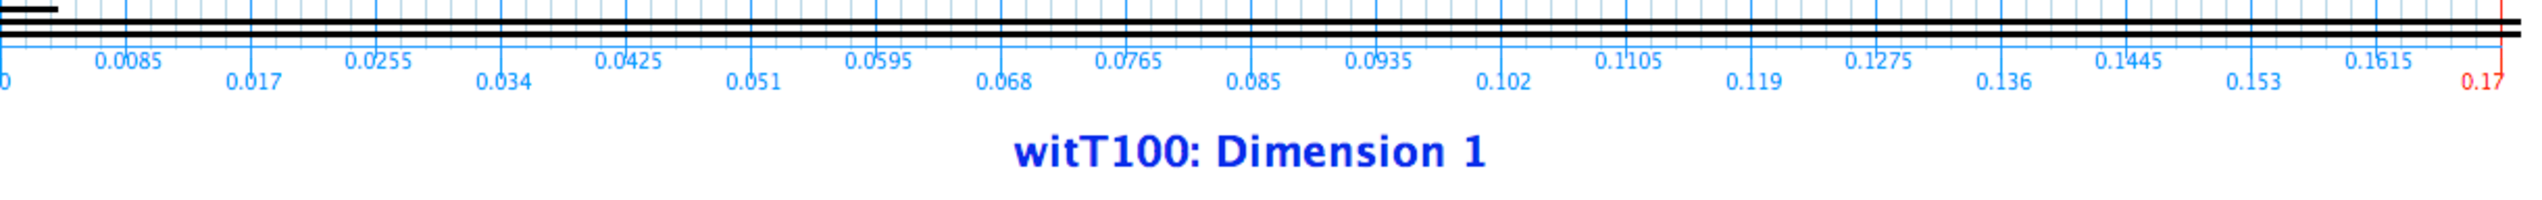
\includegraphics[width=6in]{witT100_1}}
    \subfigure{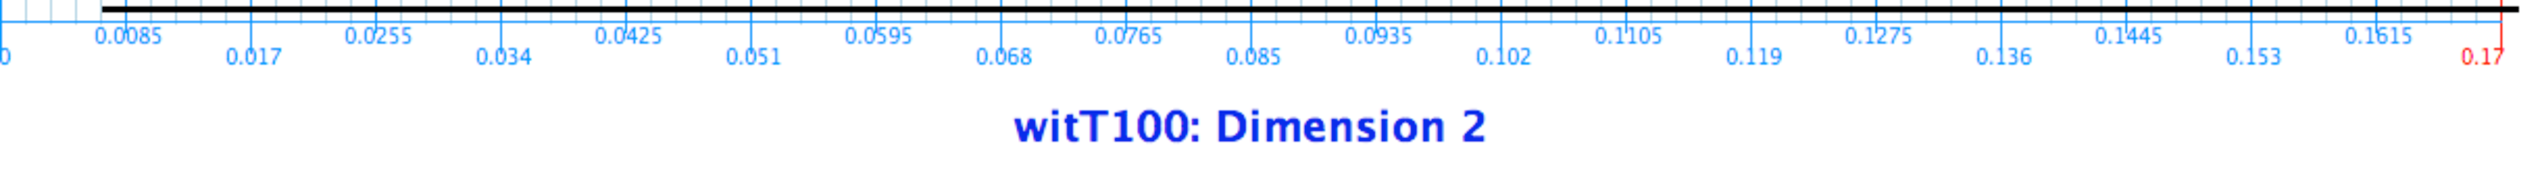
\includegraphics[width=6in]{witT100_2}}
   \end{center}
\end{figure}
\FloatBarrier

The idea of persistent homology is that long intervals should correspond to real topological features, whereas short intervals are considered to be noise. The plot above shows that for a long range, the torus numbers $Betti_0 = 1$, $Betti_1 = 2$, $Betti_2 = 1$ are obtained. Your plot should contain a similar range. \\

The WitnessStream \texttt{witT100} contains approximately 3,000 simplices, fewer than the approximately 80,000 simplices in RipsStream \texttt{ripsT20}. This is despite the fact that we started with $100^2$ points in the witness case, but only $20^2$ points in the Rips case. This supports our belief that the witness stream returns good results at lower computational expense. \\




\subsection{Subclass LazyWitnessStream}
A lazy witness stream is similar to a witness stream. However, there is an extra parameter $\nu$, typically chosen to be 0, 1, or 2, which helps determine how the lazy witness complexes $LW_\nu(Z,L,t)$ are constructed. See \cite{dsc04} for more information. \\

Suppose we are given a point cloud $Z$, landmark subset $L$, and parameter $\nu\in\mathbb{N}$. If $\nu = 0$, let $m(z) = 0$ for all $z\in Z$. If $\nu >0$, let $m(z)$ be the distance from $z$ to the $\nu$-th closest landmark point. The lazy witness complex $LW_\nu(Z,L,t)$ is defined as follows.
\begin{itemize}
\item{the vertex set is $L$.}
\item{for vertices $a$ and $b$, edge $[ab]$ is in $LW_\nu(Z,L,t)$ if there exists a witness $z \in Z$ such that $\max\bigl\{d(a,z), d(b,z)\bigr\} \leq t+m(z)$.}
\item{a higher dimensional simplex is in $LW_\nu(Z,L,t)$ if all of its edges are.} 
\end{itemize}
Note that $LW_\nu(Z,L,t) \subset LW_\nu(Z,L,s)$ whenever $t\leq s$. The adjective {\em lazy} refers to the fact that the lazy witness complex is a flag complex: since the 1-skeleton determines all higher dimensional simplices, less computation is involved. \\

\begin{exercise}
Let $Z$ be the point cloud in Figure \ref{fig:pdataHouse} from \S \ref{euc}, corresponding to PointData instance \texttt{pdataHouse}. Let $L = \{(1,0),(0,3),(-1,0)\}$ be the landmark subset. Let $\nu = 1$. Find by hand the filtration time for the edge between vertices $(1,0)$ and $(0,3)$. Which point or points witness this edge? What is the filtration time for the lone 2-simplex $[(1,0),(0,3),(-1,0)]$? \\
\end{exercise}

\begin{exercise}
Repeat the above exercise with $\nu = 0$ and with $\nu = 2$. \\
\end{exercise}

\begin{exercise}
Check that the 1-skeleton of a witness complex $W(Z,L,t)$ is the same as the 1-skeleton of a lazy witness complex $LW_2(Z,L,t)$. As a consequence, $LW_2(Z,L,t)$ is the flag complex of $W(Z,L,t)$. \\
\end{exercise}

The following sequence of commands is typical.
\begin{quote} \texttt{>> L = WitnessStream.makeRandomLandmarks(pdata, $numLands$); \index{1}{WitnessStream.makeRandomLandmarks}
} \end{quote}
\hspace{55mm} \texttt{\% Or, sequential maxmin landmarks}
\begin{quote} \texttt{>> R = WitnessStream.estimateRmax(pdata, L); \index{1}{WitnessStream.estimateRmax}\\
>> laz = Plex.LazyWitnessStream($\delta$, $d_{max}$, $t_{max}$, $\nu$, L, pdata); \index{1}{Plex.LazyWitnessStream}\\
>> intervals = Plex.Persistence.computeIntervals(laz); \index{1}{Plex.Persistence.computeIntervals}\\
>> Plex.plot(intervals, 'laz', $t_{max}$) \index{1}{Plex.plot}
} \end{quote}
Again, $t_{max}$ is often chosen in proportion to \texttt{R}. In the next section we build a lazy witness stream on a dataset of range image patches. \\




\section{Example with real data}\label{real}

We now do an example with real data. Double check that the files \texttt{pointsRange.mat} and \texttt{dct.m}, which accompany this tutorial, are in your Matlab directory. \\

In {\em On the nonlinear statistics of range image patches} \cite{ac09}, we study a space of range image patches drawn from the Brown database \cite{lpm03}. A range image is like an optical image, except that each pixel contains a distance instead of a grayscale value. Our space contains high-contrast, normalized, $5 \times5$ pixel patches. We write each $5\times5$ patch as a length 25 vector and think of our patches as point cloud data in $\mathbb{R}^{25}$. We select from this space the 30\% densest vectors, based on a density estimator called $\rho_{300}$ (see Appendix \ref{A:core}). In \cite{ac09} this dense core subset is denoted $X^5(300,30)$, and it contains 15,000 points. In the next example we verify a result from \cite{ac09}: $X^5(300,30)$ has the topology of a circle. \\

Load the file \texttt{pointsRange.mat}. The matrix \texttt{pointsRange} appears in your Matlab workspace.
\begin{quote} \texttt{>> load pointsRange.mat \\
>> size(pointsRange) \index{1}{size}\\ 
ans = 15000\ \ \ 25 \hspace{19mm} \% 15000 points in dimension 25
} \end{quote}
Matrix \texttt{pointsRange} is in fact $X^5(300,30)$: each of its rows is a vector in $\mathbb{R}^{25}$. Display some of the coordinates of \texttt{pointsRange}. It is not easy to visualize a circle by looking at these coordinates! \\

We create a PointData instance using subclass EuclideanArrayData. We pick 50 sequential maxmin landmark points, find the value of \texttt{R}, and build the lazy witness stream with parameter $\nu = 1$. 
\begin{quote} \texttt{>> pdataRange = EuclideanArrayData(pointsRange); \index{1}{EuclideanArrayData}\\
>> L = maxminLandmarks(pointsRange, 50, 'e'); \index{1}{maxminLandmarks.m}\\
>> R = WitnessStream.estimateRmax(pdataRange, L) \index{1}{WitnessStream.estimateRmax}\\
R = 0.7757\hspace{28mm} \% Generally close to 0.75 \\
>> lazRange = Plex.LazyWitnessStream(0.001, 3, R/3, 1, L, pdataRange); \index{1}{Plex.LazyWitnessStream}\\
>> lazRange.size \index{1}{size}\\
ans = 20937\hspace{26mm} \% Generally between 10000 and 25000 \\
>> intervals = Plex.Persistence.computeIntervals(lazRange);\index{1}{Plex.Persistence.computeIntervals}\\
>> Plex.plot(intervals, 'lazRange', R/3) \index{1}{Plex.plot}
} \end{quote}

\begin{figure}[htp]
  \begin{center}
    \subfigure{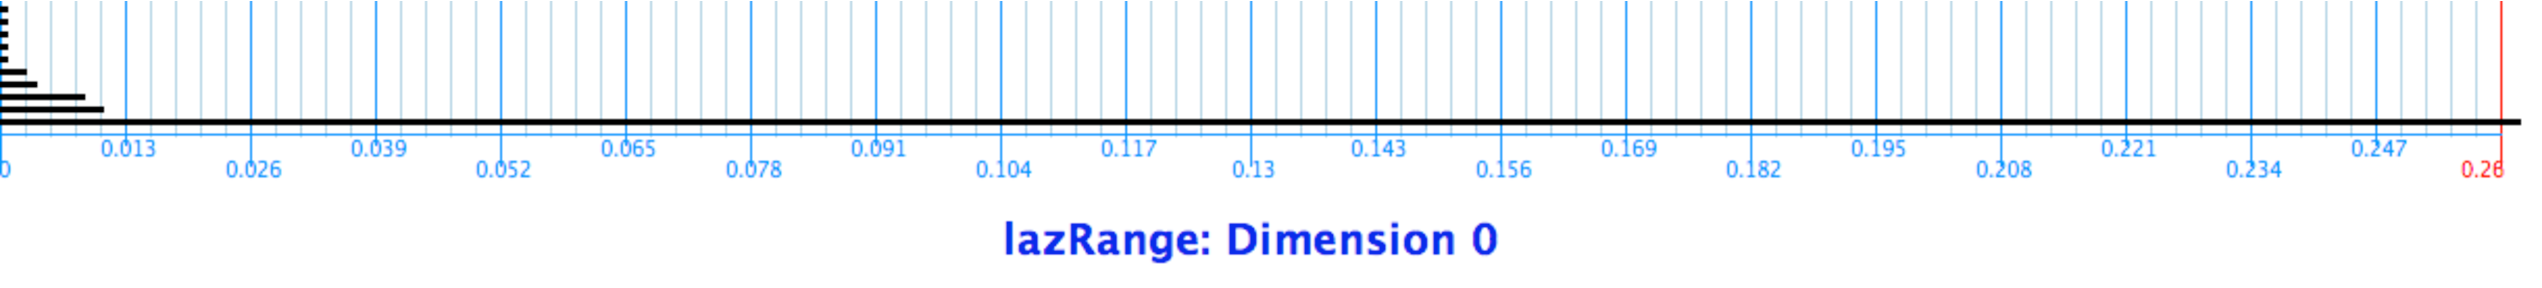
\includegraphics[width=6in]{lazRange0}}
    \subfigure{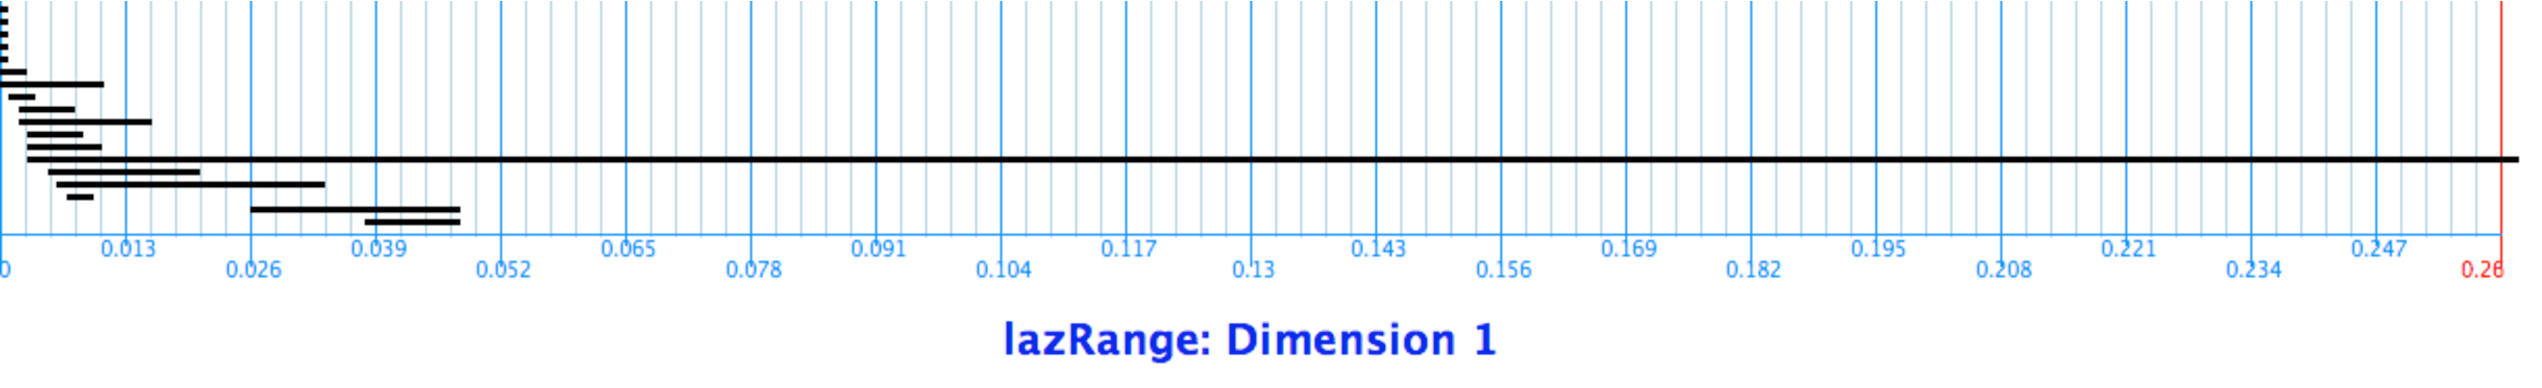
\includegraphics[width=6in]{lazRange1}}
   \end{center}
  \caption{Betti intervals for \texttt{lazRange}, built from $X^5(300,30)$}
  \label{fig:rangeBetti}
\end{figure}
\FloatBarrier

The plots above show that for a long range, the circle Betti numbers $Betti_0 = Betti_1 = 1$ are obtained. Your plot should contain a similar range. This is good evidence that the core subset $X^5(300,30)$ is well-approximated by a circle. \\

Our $5\times 5$ normalized patches are currently in the pixel basis: every coordinate corresponds to the range value at one of the 25 pixels. The Discrete Cosine Transform (DCT) basis is a useful basis for our patches \cite{ac09, lpm03}. We change to this basis in order to plot a projection of the loop evidenced by Figure \ref{fig:rangeBetti}. The method \texttt{dct.m} returns the DCT change-of-basis matrix for square patches of size specified by the input parameter.
\begin{quote} \texttt{>> pointsRangeDct = pointsRange$^*$dct(5); \index{1}{dct.m}
%>> size(pointsRangeDct)\\
%ans = 15000\quad 24 \hspace{30mm} \% 15000 points in DCT basis (representation)
} \end{quote}

Two of the DCT basis vectors are horizontal and linear gradients.

\vspace{-3mm}
\begin{figure}[htb]
	\centering
	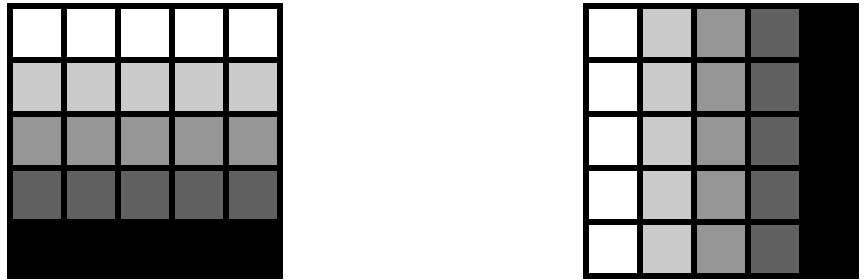
\includegraphics[width=2in]{linearGrad}
\end{figure}
\vspace{-3mm}
\FloatBarrier

We plot the projection of \texttt{pointsRangeDct} onto the linear gradient DCT basis vectors.
\begin{quote} \texttt{>> plot(pointsRangeDct(:,1), pointsRangeDct(:,5), '.'), axis square \index{1}{plot}
} \end{quote}

\begin{figure}[htp]
  \begin{center}
    \subfigure[Projection of $X^5(300,30)$]{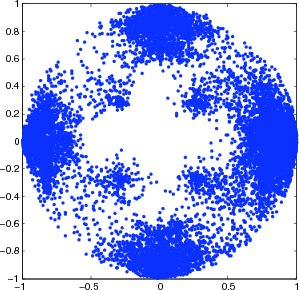
\includegraphics[width=3in]{r5k300c30}}
    \quad
    \subfigure[Range primary circle]{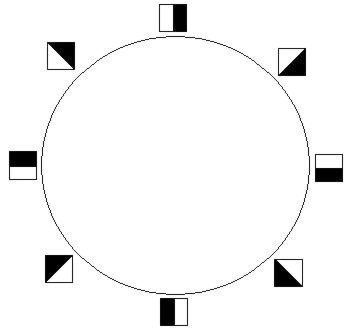
\includegraphics[width=2.9in]{primaryCircle}}
   \end{center}
\end{figure}
\FloatBarrier

The projection of $X^5(300,30)$ in Figure (a) shows a circle. It is called the range primary circle and is parameterized in Figure (b).




\section{Remarks} 

\subsection{Scripts and functions with JavaPlex commands}
In order to include JavaPlex commands in an m-file script or function, include the command \texttt{import edu.stanford.math.plex.*;} as the first command of the script. For m-file functions, include this command as the second line -  that is, as the line underneath the function header.

Writing scripts and functions is very useful. One example is the m-file \texttt{eulerCharacteristic.m}, which accepts an ExplicitStream as input and demonstrates two different methods for computing the Euler characteristic.
\begin{quote} \texttt{>> eulerCharacteristic(s6) \index{1}{eulerCharacteristic.m}\\
The Euler characteristic is 2 = 8 - 28 + 56 - 70 + 56 - 28 + 8, using the alternating sum of cells.\\
The Euler characteristic is 2 = 1 - 0 + 0 - 0 + 0 - 0 + 1, using the alternating sum of Betti numbers.} \end{quote}




\subsection{Representative cycles}
The persistence algorithm that computes barcodes can also find a representative cycle for each homology class. The current version of JavaPlex does not return representative cycles, though development versions of JavaPlex can. There is no guarantee that the produced representative will be geometrically nice. 




\subsection{Java heap size}
Depending on the size of your JavaPlex computations, you may need to increase the maximum Java heap size. This should not be necessary for the examples in this tutorial. \\

The following command returns your maximum heap size in bytes.
\begin{quote} \texttt{>> java.lang.Runtime.getRuntime.maxMemory \index{1}{java.lang.Runtime.getRuntime.maxMemory}\\
ans = 130875392
} \end{quote}
My computer has a heap limit of approximately 128 megabytes. To increase your limit to, say, 256 megabytes, create a file named \texttt{java.opts} in your Matlab directory which contains the text \texttt{-Xmx256m} and then restart Matlab.




\subsection{From Java variables to Matlab variables}
Some JavaPlex commands return Java variables, when instead one might want output in the form of a Matlab variable, such as a matrix of numbers. One way to transform Java variables into Matlab variables is by using an m-file. For instance, in \S \ref{explicitStream} we used the m-file \texttt{interval2mat.m} to take an array of type PersistenceInterval into a Matlab matrix. Similarly, the m-file \texttt{betti2mat.m} accepts input of type \texttt{Plex.BettiNumbers} and returns a Matlab vector of integers. These commands are typically used as shown below, where \texttt{intervals} is an array of type PersistenceInterval.

\begin{quote} \texttt{>> intervalMatrix = interval2mat(intervals); \index{1}{interval2mat.m}\\
>> bettiVect = betti2vect(Plex.FilterInfinite(intervals)); \index{1}{betti2vect.m}\index{1}{FilterInfinite}\\
} \end{quote}




\appendix
\appendixpage
\addappheadtotoc




\section{Dense core subsets}\label{A:core}

A core subset of a dataset is a collection of the densest points, such as $X^5(300,30)$ in \S \ref{real}. Since there are many density estimators, and since we can choose any number of the densest points, a dataset has a variety of core subsets. In this appendix we discuss how to create core subsets. \\

Real datasets can be very noisy, and outlier points can signi�cantly alter the computed topology. Therefore, instead of trying to approximate the topology of an entire dataset, we often proceed as follows. We create a family of core subsets and identify their topologies. Looking at a variety of core subsets can give a good picture of the entire dataset. \\

See \cite{cidsz08, dsc04} for an example using multiple core subsets. The dataset is high-contrast patches from natural images. The authors use three density estimators. As they change from the most global to the most local density estimate, the topologies of the core subsets change from a circle, to three intersecting circles, to a Klein bottle. \\

One way to estimate the density of a point $z$ in a point cloud $Z$ is as follows. Let $\rho_k(z)$ be the distance from $z$ to its $k$-th closest neighbor. Let the density estimate at $z$ be $\frac{1}{\rho_k(z)}$. Varying parameter $k$ gives a family of density estimates. Using a small value for $k$ gives a local density estimate, and using a larger value for $k$ gives a more global estimate. \\

For Euclidean datasets, one can use the m-file \texttt{kDensitySlow.m} to produce density estimates $\frac{1}{\rho_k}$. The following command is typical.
\begin{quote} \texttt{>> densities = kDensitySlow(points, $k$); \index{1}{kDensitySlow.m}
} \end{quote}
Input \texttt{points} is an $N\times n$ matrix of $N$ points in $\mathbb{R}^n$. Input $k$ is the density estimate parameter. Output \texttt{densities} is a vertical vertex of length $N$ containing the density estimate at each point. \\

M-file \texttt{coreSubset.m} builds a core subset. The following command is typical.
\begin{quote} \texttt{>> core = coreSubset(points, densities, numPoints); \index{1}{coreSubset.m}
} \end{quote}
Inputs \texttt{points} and \texttt{densities} are as above. Output \texttt{core} is a $\texttt{numPoints}\times n$ matrix representing the \texttt{numPoints} densest points. \\

{\em Prime numbers example.} The command \texttt{primes(3571)} returns a vector listing all prime numbers less than or equal to 3571, which is the 500-th prime. We think of these primes as points in $\mathbb{R}$ and build the core subset of the 10 densest points with density parameter $k = 1$.
\begin{quote} \texttt{>> p = primes(3571)'; \index{1}{primes}\\
>> length(p) \index{1}{length}\\
ans = 500 \\
>> densities1 = kDensitySlow(p, 1); \index{1}{kDensitySlow.m}\\
>> core1 = coreSubset(p, densities1, 10) \index{1}{coreSubset.m}\\
core1 =
} \end{quote}

\hspace{15mm} \texttt{2}

\hspace{15mm} \texttt{3}

\hspace{15mm} \texttt{5}

\hspace{15mm} \texttt{7}

\hspace{15mm} \texttt{11}

\hspace{15mm} \texttt{13}

\hspace{15mm} \texttt{17}

\hspace{15mm} \texttt{19}

\hspace{15mm} \texttt{29}

\hspace{15mm} \texttt{31} \\
We get a bunch of twin primes, which makes sense since $k = 1$. Let's repeat with $k = 50$.
\begin{quote} \texttt{>> densities50 = kDensitySlow(p, 50); \index{1}{kDensitySlow.m}\\
>> core50 = coreSubset(p, densities50, 10) \index{1}{coreSubset.m}\\
core50 =
} \end{quote}

\hspace{15mm} \texttt{113}

\hspace{15mm} \texttt{127}

\hspace{15mm} \texttt{109}

\hspace{15mm} \texttt{131}

\hspace{15mm} \texttt{107}

\hspace{15mm} \texttt{137}

\hspace{15mm} \texttt{139}

\hspace{15mm} \texttt{157}

\hspace{15mm} \texttt{149}

\hspace{15mm} \texttt{151} \\
With $k = 50$, we expect the densest points to be slightly larger than the 25-th prime, which is 97. \\

{\em Note:} As its name suggests, the m-file \texttt{kDensitySlow.m} is not the most efficient way to calculate $\rho_k$ for large datasets. There is a faster file \texttt{kDensity.m} for this purpose, which uses the kd-tree data structure. I have not included it in the tutorial because it requires one to download a kd-tree package for Matlab, available at \url{http://www.mathworks.com/matlabcentral/fileexchange/21512-kd-tree-for-matlab}. Please email me at \texttt{henrya@math.stanford.edu} if you're interested in using \texttt{kDensity.m}.

% What are the differences in timings between fast and slow versions?
% It seems that k=300 is surprisingly slow with kDensity.m: 1108 seconds. Slower than kDensitySlow.m. Double check?

%I typically use the m-file \texttt{kDensitySlow.m} on datasets of around 50,000 points (for instance, $X^5(300,30)$ in \S \ref{real} is the 30\% densest points from a set of size 50,000, using the density estimate $\rho_{300}$). This computation takes about 10 minutes on my MacBook, which is much longer than any of the computations I do using the JPlex software. \\ % Elapsed time is 432.024880 seconds, 7-17-09. This was effectively kDensitySlow.m, I think




%\printindex{1}{Index of JavaPlex and Matlab commands}
% terminal command to compile index: 
% cd Desktop/JPlexTutorials/PlexMatlabTutorial
% makeindex 1

\begin{thebibliography}{9}

\bibitem{ac09}
{\sc H.~Adams and G.~Carlsson}, {\em On the nonlinear statistics of range image patches}, SIAM J. Img. Sci., 2, (2009), pp.~110-117.
	
\bibitem{a83}
{\sc M.~A.~Armstrong}, {\em Basic Topology}, Springer, New York, Berlin, 1983.

\bibitem{cidsz08}
{\sc G.~Carlson, T.~Ishkhanov, V.~de Silva, and A.~Zomorodian}, {\em On the local behavior of spaces of natural images}, Int. J. Computer Vision, 76 (2008), pp.~1--12.

\bibitem{dsc04}
{\sc V.~de Silva and G.~Carlsson}, {\em Topological estimation using witness complexes}, in Proceedings of the Symposium on Point-Based Graphics, ETH, Z\"urich, Switzerland, 2004, pp.~157--166.

\bibitem{eh10}
{\sc H.~Edelsbrunner and J.~Harer}, {\em Computational Topology: An Introduction}, American Mathematical Society, Providence, 2010.

\bibitem{elz02}
{\sc H.~Edelsbrunner, D.~Letscher, and A.~Zomorodian}, {\em Topological persistence and simplification},  Discrete Computat. Geom., 28 (2002), pp.~511--533.

\bibitem{h02}
{\sc A.~Hatcher}, {\em Algebraic Topology}, Cambridge University Press, Cambridge, UK, 2002.

\bibitem{lpm03}
{\sc A.~B.~Lee, K.~S.~Pedersen, and D.~Mumford}, {\em The nonlinear statistics of high-contrast patches in natural images}, Int. J. Computer Vision, 54 (2003), pp.~83--103.

\bibitem{jplex}
{\sc H.~Sexton and M.~Vejdemo-Johansson}, JPlex simplicial complex library. \url{http://comptop.stanford.edu/programs/jplex/}.

\bibitem{zc05}
{\sc A. Zomorodian and G. Carlsson}, {\em Computing persistent homology}, Discrete Computat. Geom., 33 (2005), pp.~247--274. 

\end{thebibliography}

\end{document}
